\section{RL Algorithms}

\begin{frame}{Value Iteration: model-based approach}
  \begin{itemize}
  \item KRk: 182.676 states
  \item Feasible number of states + perfect knowledge $\rightarrow$ Dynamic Programming
  \item $V(s) \leftarrow \max_a \sum_{s',r}p(s',r'|s,a)[r(s,a,s')+\gamma V(s')]$
  \item $\pi(s) = \arg\max_a \sum_{s',r}p(s'|s,a)[r(s,a,s')+\gamma V(s')]$
  \end{itemize}
\end{frame}

\begin{frame}{Choice of parameters}
  \begin{itemize}
    \item Step penalty: -2 $\rightarrow$ values = DTZ
    \item Draw penalty: -100 $\rightarrow$ slow mates > quick draws
    \item $\gamma = 1$
    \item $\theta = 0.0001$
  \end{itemize}
  % 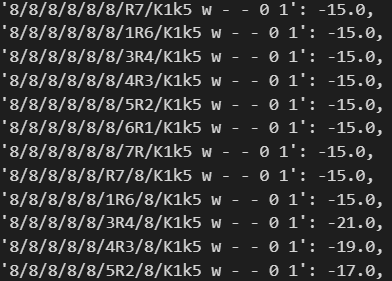
\includegraphics[width=0.7\textwidth]{images/DTZ_values.png}
\end{frame}

% \begin{frame}{Random Player}
%   \begin{itemize}
%     \item Idea: how much different is the policy learned against a random player?
%     \item Applied Value Iteration with uniform random black defender
%     \item Applied Q-Learning with uniform random black defender 
%   \end{itemize}
% \end{frame}

\begin{frame}{Q-Learning: model-free approach}
  \begin{itemize}
    \item How good of a policy without knowing the ``level" of the opponent?
    \item $Q(s,a) \leftarrow Q(s,a) + \alpha[r + \gamma \max_{a'}Q(s',a') - Q(s,a)]$
    \item $\pi(s) = \arg\max_a Q(s,a)$
    \item Off-policy, online and one-step.
  \end{itemize}
\end{frame}

\begin{frame}{Choice of parameters}
  \begin{itemize}
    \item \textbf{Max steps} per episode: 50 $\rightarrow$ if it's too far from mate, agent may never reach terminal state
    \item Step penalty: -0.01
    \item Draw penalty: -1
    \item $\gamma = 0.99$
    \item Costant learning rate $\alpha = 0.05$ $\rightarrow$ smaller variance
    \item $\epsilon$-greedy policy with $\epsilon = 0.3$ with decay
  \end{itemize}
\end{frame}

\begin{frame}{Actor-critic: approximate solution approach}
  \begin{itemize}
    \item Non-elementary chess endgames $\rightarrow$ \textbf{curse of dimensionality}
    \item Use one-step actor-critic
    \item Update rules:
    \begin{itemize}
      \item $\delta = r + \gamma V(s';w) - V(s;w)$
      \item $\theta \leftarrow \theta + \alpha^{\theta} \delta \nabla_{{\theta}} \log \pi(a|s;\theta) $
      \item $w \leftarrow w + \alpha^{w} \delta \nabla_w V(s;w)$
    \end{itemize} 
  \end{itemize}
\end{frame}

\begin{frame}{Parameters Choice}
\begin{itemize}
    \item Policy: MLP(128,128,64), ReLU activations, softmax output 
    \item Value function: $V(s) = \sum_{i=1}^{16} w_i \phi_i(s)$
    \item parameters: %TODO
\end{itemize}
\end{frame}

\begin{frame}{Feature engineering}
  % \begin{itemize}
  %   \item Feature engineering:
  %   \begin{itemize}
  %     \item Manhattan distance between kings
  %     \item Manhattan distance between black king and white rook 
  %     \item File and rank of the kings
  %     \item Distance of the Black King from the side of the board
  %     \item Binary indicator of opposition, parity 
  %   \end{itemize}
  % \end{itemize}

  \begin{figure}
    \centering
    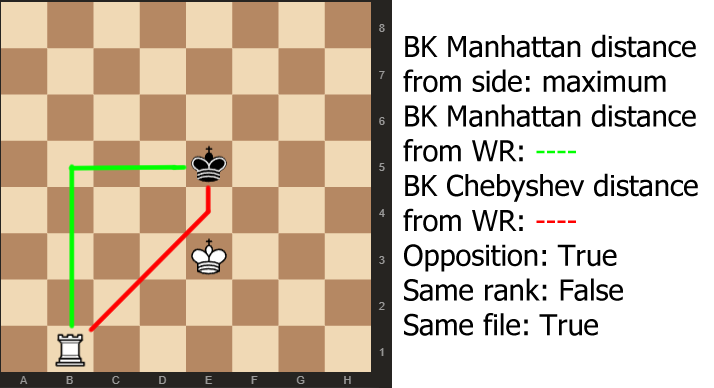
\includegraphics[width=0.8\textwidth]{images/features.png}
  \end{figure}
\end{frame}



\begin{frame}{Monte Carlo Tree Search}
  \begin{itemize}
    \item One of the first methods to solve chess
    \item No need to train!
    \item Heuristic method
  \end{itemize}
\end{frame}